\documentclass[hyperref, notheorems]{beamer}

% PACKAGES
\usepackage[utf8]{inputenc}
\usepackage{geometry}
\usepackage{appendix}
\usepackage{ytableau}
\usepackage{hyperref}
\usepackage{amsmath}
\usepackage{amssymb}
\usepackage{amsthm}
\usepackage{mathrsfs}
\usepackage{tcolorbox}
\usepackage{pgf}
\usepackage{tikz}
\usepackage{tikz-cd}
\usetikzlibrary{arrows,decorations.markings}
\usepackage{pst-platon}
\usepackage{transparent}
\usepackage{graphicx}
\usepackage{xcolor}

% NEW ENVIRONMENTS
\newenvironment{reference}{\begin{tcolorbox}[width=\linewidth,baseline=\tcbtextheight+\baselineskip]}{\end{tcolorbox}}
\newenvironment{creference}{\begin{tcolorbox}[width=\linewidth,baseline=\tcbtextheight+\baselineskip]\centering}{\end{tcolorbox}}

% NEW AND REDEFINED COMMANDS
\newcommand{\legendre}[2]{\genfrac{(}{)}{0.5pt}{0}{#1}{#2}}
\newcommand{\tmod}[1]{\text{ mod }#1}
\newcommand{\xto}[1]{\xrightarrow{#1}}
\newcommand{\xfrom}[1]{\xleftarrow{#1}}
\newcommand{\normal}{\mathrel{\unlhd}}
\newcommand{\mf}[1]{\mathfrak{#1}}
\newcommand{\Mat}{\mathrm{Mat}}
\newcommand{\GL}{\mathrm{GL}}
\newcommand{\SL}{\mathrm{SL}}
\renewcommand{\O}{\mathrm{O}}
\newcommand{\N}{\mathbb{N}}
\newcommand{\Z}{\mathbb{Z}}
\newcommand{\Q}{\mathbb{Q}}
\newcommand{\R}{\mathbb{R}}
\newcommand{\C}{\mathbb{C}}
\newcommand{\F}{\mathbb{F}}
\renewcommand{\H}{\mathbb{H}}
\renewcommand{\P}{\mathbb{P}}
\renewcommand{\a}{\alpha}
\renewcommand{\b}{\beta}
\newcommand{\g}{\gamma}
\renewcommand{\d}{\delta}
\newcommand{\e}{\epsilon}
\newcommand{\z}{\zeta}
\renewcommand{\t}{\theta}
\renewcommand{\i}{\iota}
\renewcommand{\k}{\kappa}
\renewcommand{\l}{\lambda}
\newcommand{\s}{\sigma}
\renewcommand{\o}{\omega}
\newcommand{\vphi}{\varphi}
\newcommand{\emt}{\varnothing}
\newcommand{\x}{\times}
\newcommand{\ox}{\otimes}
\newcommand{\op}{\oplus}
\newcommand{\del}{\partial}
\DeclareMathOperator{\id}{\textrm{id}}
\DeclareMathOperator{\sgn}{\mathrm{sgn}}
\DeclareMathOperator{\im}{\mathrm{im}}
\DeclareMathOperator{\rk}{\mathrm{rk}}
\DeclareMathOperator{\tr}{\mathrm{trace}}
\DeclareMathOperator{\ord}{\mathrm{ord}}
\DeclareMathOperator{\Hom}{\mathrm{Hom}}
\DeclareMathOperator{\End}{\mathrm{End}}
\DeclareMathOperator{\Aut}{\mathrm{Aut}}
\DeclareMathOperator{\Tor}{\mathrm{Tor}}
\DeclareMathOperator{\Ann}{\mathrm{Ann}}
\DeclareMathOperator{\Gal}{\mathrm{Gal}}
\DeclareMathOperator{\Trace}{\mathrm{Trace}}
\DeclareMathOperator{\Norm}{\mathrm{Norm}}
\usepackage{quiver}
\newcommand{\afrak}{\mathfrak{a}}
\newcommand{\Rbb}{\mathbb{R}}
\newcommand{\Zbb}{\mathbb{Z}}
\newcommand{\Pbb}{\mathbb{P}}
\newcommand{\Cbb}{\mathbb{C}}
\newcommand{\Abb}{\mathbb{A}}
\newcommand{\Vbb}{\mathbb{V}}
\newcommand{\txtblue}{\textcolor{blue}}
\newcommand{\Ydd}{Y_{\Tilde{\Delta} /\Delta}}
\usepackage{mathtools}
% BACK OF POCKET TOOLS
% [label=(\roman*)]
% [label=(\alph*)]
% [label=(\arabic{enumi})]


% SPECIAL COMMANDS
\newcommand{\smathcal}[1]{
    \mathchoice
    {{\scriptstyle\mathcal{#1}}}
    {{\scriptstyle\mathcal{#1}}}
    {{\scriptscriptstyle\mathcal{#1}}}
    {\scalebox{.7}{$\scriptscriptstyle\mathcal{#1}$}}
}

% TIKZ PREAMBLE
\newcommand{\disc}{\draw(0,0) [fill=gray] circle (1cm);}
\newcommand{\strip}[1]{
\fill [white,even odd rule,rotate=#1] (1,0) circle[radius=0.42cm] circle[radius=0.28cm];
\fill [lightgray,even odd rule,rotate=#1] (1,0) circle[radius=0.4cm] circle[radius=0.3cm];}
\newcommand{\varstrip}[3]{
\fill [white,even odd rule,rotate=#1] (1,0) circle[radius=0.3*#2+0.12*#3] circle[radius=0.3*#2-0.02*#3];
\fill [lightgray,even odd rule,rotate=#1] (1,0) circle[radius=0.3*#2+0.1*#3] circle[radius=0.3*#2];}
\newcommand{\mstrip}[1]{
\fill [white,rotate=#1] (0.8,0.38) -- (1.25, 0.23) -- (1.43,0.1) -- (1.43,-0.1) -- (1.25,-0.23) -- (0.8,-0.38) -- (0.8,-0.22) -- (1,-0.17) -- (1.3,-0.05) -- (1.3,0.05) -- (0.8,0.22) -- (1,0.17) -- cycle;
\draw [thick,domain=-0.4:0.4,rotate=#1+2.5] plot ({1.4-7*\x*\x}, {\x});
\fill [white,rotate=#1] (1.36,0.01) circle(0.04);
\draw [thick,domain=-0.4:0.4,rotate=#1-2.5] plot ({1.4-7*\x*\x}, {\x});
}
\tikzset{vertex/.style = {shape=circle,draw,minimum size=1.5em}}
\tikzset{edge/.style = {->,> = latex'}}
\tikzset{->-/.style={decoration={
  markings,
  mark=at position 0.55 with {\arrow{stealth}}},postaction={decorate}}}

%BEAMER PREAMBLE
\usefonttheme[onlymath]{serif}
\definecolor{burgundy}{rgb}{0.5, 0.0, 0.13}
\usetheme[sidebarleft]{Caltech}
\setbeamertemplate{footline}[frame number]
\setbeamercovered{transparent}
\theoremstyle{definition}
\newtheorem{definition}{\translate{Definition}}
\newtheorem{theorem}{\translate{Theorem}}
\newtheorem{example}{\translate{Example}}
\newtheorem{conjecture}{\translate{Conjecture}}

% TITLE
\title{Rationality of Real Conic Bundles with Quartic Discriminant Curve}
\author{Mattie Ji}
\institute{Brown University}
\date{Advised by Lena Ji\\ 2022 Mathematics REU Program - University of Michigan}
\AtBeginSection[]{
  \begin{frame}
    \frametitle{Outline}
    \tableofcontents[currentsection]
  \end{frame}
}

%Table of Content

\begin{document}

\begin{frame}
    \titlepage
\end{frame}

% \begin{frame}
%     \frametitle{Outline}
%     \tableofcontents
% \end{frame}

% Hide subsections from table of contents
% \begin{frame}{Outline}
%     \tableofcontents[hideallsubsections]
% \end{frame}
% https://latex-beamer.com/tutorials/table-of-contents/

% Presentation structure
\section{Background}


% \section*{References}

\begin{frame}{Notations}
    Throughout this talk,
    \begin{itemize}
        \item Unless otherwise specified, we will work over $\Rbb$ as our ground field
        \item We will denote the projective n-space over the ground field as $\Pbb^n$
        \item Sometimes, to emphasize the coordinates $[X_0 :\ ...\ : X_n]$ of $\Pbb^n$, we will denote $\Pbb^n$ as $\Pbb^n_{[X_0 :\ ...\ : X_n]}$
    \end{itemize}
\end{frame}

    \subsection{Plane Conics}

\begin{frame}{Overview of Conics}
    \begin{itemize}
        \item A \txtblue{plane conic} $C \subset \Pbb^2$ is the curve defined 
        \[C \coloneqq (F(X, Y, Z) = 0)\]
        where $F(X, Y, Z) = a X^2 + b Y^2 + c Z^2 + d XY + e YZ + f XZ$ is a homogeneous polynomial of degree $2$ in $\Rbb[X, Y, Z]$ 
        \item This $C$ has an associated \txtblue{symmetric matrix $M_F$}
        \[M_F \coloneqq \begin{bmatrix}
        a & \frac{d}{2} & \frac{f}{2}\\
        \frac{d}{2} & b & \frac{e}{2}\\
        \frac{f}{2} & \frac{e}{2} & c
        \end{bmatrix}\]
        such that
        \[F(X, Y, Z) = \begin{bmatrix} 
        X & Y & Z
        \end{bmatrix}
        M_F
        \begin{bmatrix} 
        X\\
        Y\\
        Z
        \end{bmatrix}\]
        \item $C$ is \txtblue{smooth} if and only if $M_F$ has \txtblue{rank $3$}
    \end{itemize}
\end{frame}

    \subsection{Conic Bundles}
    
\begin{frame}{Conic Bundles}
    
\begin{block}{Definition:}
A \textbf{conic bundle} over $\Pbb^2$ is a ``nice"\footnote{A proper flat $\Rbb$-morphism} morphism $\pi: X \to \Pbb^2$ such that 
\begin{itemize}
    \item $X$ is a smooth variety
    \item The fiber over every point $p \in \Pbb^2$ is a conic
    \item The generic fiber is a smooth conic
\end{itemize}
\end{block}
\end{frame}

\begin{frame}{Conic Bundles}
    In our research, we are interested in the \txtblue{conic bundle $\pi_2: \Ydd \to \Pbb^2_{[u: v: w]}$} where:
    \begin{itemize}
        \item $\Ydd$ is a variety defined by the equation\footnote{This looks like a very specific choice, but it turns out that every degree $4$ conic bundle $X \to \Pbb^2$ is birationally equivalent to some $\pi_2$ ``up to a class in $\Zbb/2\Zbb$" (Theorem 2.6 of \cite{FJSVV} based on \cite{bruin})}:
    \[z^2 = Q_1(u, v, w) t_0^2 + 2Q_2(u, v, w) t_0t_1 + Q_3(u, v, w) t_1^2\]
        \item $Q_1, Q_2, Q_3 \in \Rbb[u, v, w]$ are homogenous polynomials of degree $2$
        \item $\pi_2$ is the standard projection that forgets $z, t_0, $ and $t_1$
    \end{itemize}
    We are also interested in the map \txtblue{$\pi_1: \Ydd \to \Pbb^1_{[t_0: t_1]}$}, which is the standard projection that forgets $z, u, v,$ and $w$.
\end{frame}

\begin{frame}{Why is $\pi_2$ a conic bundle?}
Intuitively, every point in $\Pbb^2$ should correspond to some conic in $\Ydd$. 
    \begin{block}{Example of Fibers for $\pi_2$:}
    Concretely, take the point ${\color{red}[1 : 2 : 3]} \in \Pbb^2_{[u:v:w]}$, then fiber of ${\color{red}[1 : 2 : 3]}$ is exactly the solutions satisfying:
    \[0 = Q_1({\color{red}1, 2, 3})\colorbox{yellow}{$t_0^2$} + 2Q_2({\color{red}1, 2, 3})\colorbox{yellow}{$t_0t_1$} + Q_3({\color{red}1, 2, 3})\colorbox{yellow}{$t_1^2$} - \colorbox{yellow}{$z^2$}\]
    This forms a conic in $\Pbb^2_{[t_0:t_1:z]}$.
    \end{block}
\end{frame}

\begin{frame}{Conic Bundles}
    Putting $\pi_1$ and $\pi_2$ together, we have the commutative diagram:
        \[\begin{tikzcd}[ampersand replacement=\&]
	\& {Y_{\tilde{\Delta}/\Delta}} \\
	\& {\mathbb{P}^1_{[t_0:t_1]} \times \mathbb{P}^2_{[u:v:w]}} \\
	{\mathbb{P}^1_{[t_0:t_1]}} \&\& {\mathbb{P}^2_{[u:v:w]}}
	\arrow[from=1-2, to=2-2]
	\arrow[from=2-2, to=3-1]
	\arrow["{\pi_1}"', curve={height=12pt}, from=1-2, to=3-1]
	\arrow[from=2-2, to=3-3]
	\arrow["{\pi_2}", curve={height=-12pt}, from=1-2, to=3-3]
\end{tikzcd}\]
In this talk, we refer to this as the \textbf{double cover model}.
\end{frame}

\begin{frame}{Conic Bundles}
    This commutative diagram also induces a diagram between \textbf{their real points}:
            \[\begin{tikzcd}[ampersand replacement=\&]
	\& {Y_{\tilde{\Delta}/\Delta}(\Rbb)} \\
	\& {\mathbb{P}^1_{[t_0:t_1]}(\mathbb{R}) \times \mathbb{P}^2_{[u:v:w]}(\mathbb{R})} \\
	{\mathbb{P}^1_{[t_0:t_1]}(\mathbb{R})} \&\& {\mathbb{P}^2_{[u:v:w]}(\mathbb{R})}
	\arrow[from=1-2, to=2-2]
	\arrow[from=2-2, to=3-1]
	\arrow["{\pi_1(\Rbb)}"', curve={height=12pt}, from=1-2, to=3-1]
	\arrow[from=2-2, to=3-3]
	\arrow["{\pi_2(\Rbb)}", curve={height=-12pt}, from=1-2, to=3-3]
\end{tikzcd}\]
\end{frame}

% \begin{frame}{The Discriminant Curve}
% We would like to identify if a given fiber of $\pi_2$ is smooth:
%     \begin{block}{Smoothness Criterion}
%        Given fixed $[u: v: w] \in \Pbb^2_{[u: v: w]}(\Rbb)$, we can rewrite its assoicated conic as:
%        \[0 = {\color{red}Q_1(u, v, w)}t_0^2 + {\color{red}2Q_2(u, v, w)}t_0t_1 + {\color{red}Q_3(u, v, w)}t_1^2 + {\color{red}(-1)}z^2\ (*)\]
%        This gives the symmetric matrix:
%        \[M = \begin{bmatrix}
%        Q_1(u, v, w) & Q_2(u, v, w) & 0\\
%        Q_2(u, v, w) & Q_3(u, v, w) & 0\\
%        0 & 0 & -1
%        \end{bmatrix}\]
%        The conic $(*)$ is smooth if and only if $\det(M) \neq 0$.
%     \end{block}
% \end{frame}

\begin{frame}{The Discriminant Curve}
    \begin{block}{Smoothness Criterion:}
    Let $M$ be the symmetric matrix associated to each conic of $\Ydd$, the curve defined by $\det(M) = 0$ is called the \textbf{discriminant curve} $\Delta$:
    \[\Delta = (Q_1Q_3 - Q_2^2 = 0) \subset \Pbb^2_{[u: v: w]}\]
    The fiber of $s \in \Pbb^2_{[u: v: w]}$ is smooth if and only if $s \notin \Delta$
    \end{block}

\begin{figure}[h]
    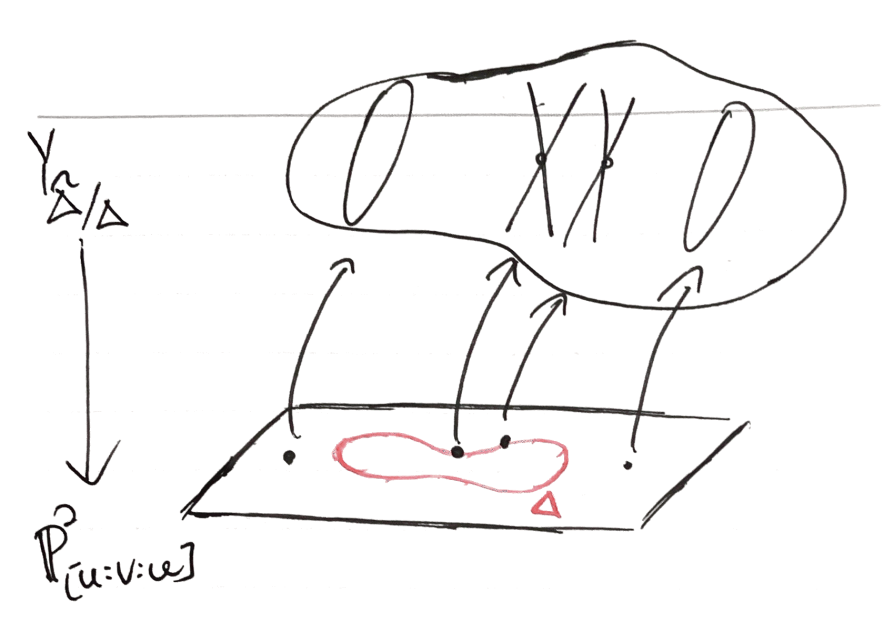
\includegraphics[width=5cm]{graphics/conic_bundle.png}
\end{figure}
\end{frame}

\begin{frame}{The Double Cover of $\Delta$}
    \begin{block}{Fact:}
        There exists a curve $\Tilde{\Delta} \subset \Pbb^4_{[u:v:w:r:s]}$ defined by
        \[\tilde{\Delta} \coloneqq (Q_1 - r^2 = Q_2 - rs = Q_3 - s^2 = 0)\]
        such that the projection $\Tilde{\Delta} \to \Delta$ is a double cover.\\ $\Tilde{\Delta}$ is called the \textbf{double cover} of $\Delta$. 
    \end{block}
    \begin{figure}[h]
    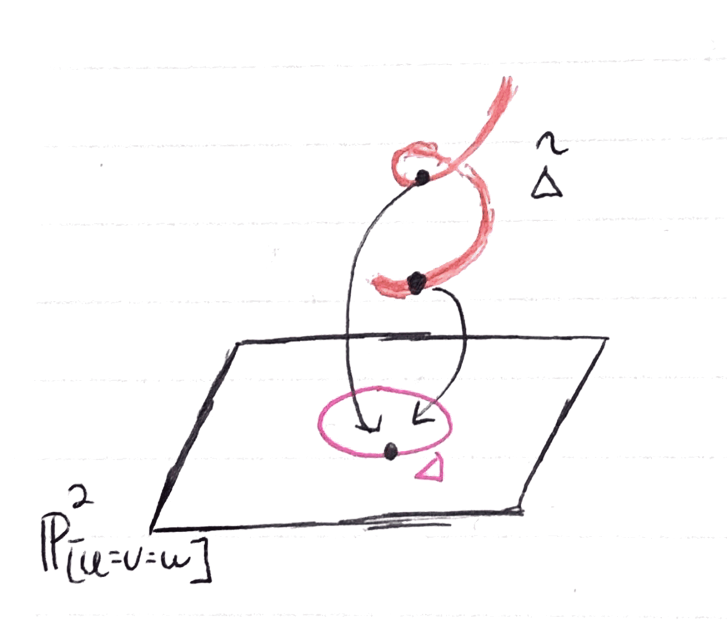
\includegraphics[width=5cm]{graphics/double_cover.png}
\end{figure}
\end{frame}

\subsection{Real Quartic Plane Curves}

\begin{frame}{Quartic Plane Curves}
$Q_1Q_3 - Q_2^2$ is a degree 4 homogeneous real polynomial.
\begin{definition}
The roots of a degree 4 homogenous polynomial over $\Pbb^2$ is known as a \textbf{quartic}.
\end{definition}
        \begin{block}{Theorem (Zeuthen, 1874 \cite{Zeuthen1874})}
       Let $\Delta$ be a smooth quartic over $\Rbb$, then $\Delta(\Rbb)$ can be classified into 1 of the 6 following topological types:
       \begin{enumerate}
           \item No real points
           \item One oval
           \item Two nested ovals
           \item Two non-nested ovals
           \item Three ovals
           \item Four ovals
       \end{enumerate}
        \end{block}
\end{frame}

\begin{frame}{Example: Four Ovals}

 The homogeneous equation defines a smooth quartic whose real component has 4 ovals:
 \[0 = -11u^4 - 5u^2 v^2 - 2 v^4 + 11 u^2 w^2 + 4 v^2 w^2 - 3 w^4\]
The real components on the chart $(w \neq 0)$
 \[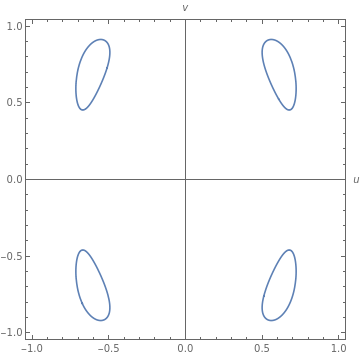
\includegraphics[width=5cm]{graphics/4ovals.png}\]
    
\end{frame}

\begin{frame}{Example: Two Nested Ovals}
This homogeneous equation defines a smooth quartic whose real component has 2 nested ovals:
 \[0 = -3u^4 - \frac{7}{10}u^2v^2 - \frac{169}{400}v^4 + \frac{67}{6}u^2w^2 + \frac{949}{240}v^2w^2 - \frac{121}{576}w^4\]
The real components on the chart $(w \neq 0)$:
 \[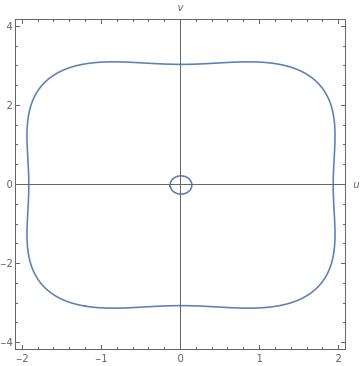
\includegraphics[width=5cm, height=5cm]{graphics/nested.png}\]
\end{frame}

\subsection{Rationality}
    
\begin{frame}{Overview of Rationality}
\begin{itemize}
    \item A variety $X$ is \txtblue{$k$-rational} over a field $k$ if there exists non-empty open sets $U \subset X$ and $V \subset \Pbb^{\dim X}_k$ such that $U$ and $V$ are isomorphic over $k$.
    \item If $X$ is not rational over $k$, we say that $X$ is \txtblue{irrational} over $k$.
\end{itemize}

There are two relevant facts about rationality:
\begin{itemize}
    \item \textbf{Lang–Nishimura Lemma: } If $X$ is a projective $k$-rational variety, then $X(k)$ is non-empty.
    \item \textbf{General Topological Fact: } If $X$ is a smooth projective $\Rbb$-rational variety, then $X(\Rbb)$ is connected.
\end{itemize}

In particular,
\[\Ydd \text{ is $\Rbb$-rational} \implies \text{$\Ydd(\Rbb)$ is non-empty and connected}\]
\end{frame}

\begin{frame}{Criterion for Rationality}
The $\Cbb$-rationality of $\Ydd$ is quite clear:

\begin{block}{Theorem (Iskovskikh, 1987 \cite{Iskovskikh-rationality-cbs})}
    $\Ydd$ is always $\Cbb$-rational
\end{block}
The $\Rbb$-rationality of $\Ydd$ is more complicated, but the work of S. Frei, L. Ji, S. Sankar, B. Viray, and I. Vogt previously gave a very useful criterion:
\begin{block}{Proposition (Proposition 6.1, \cite{FJSVV})}
    Let $\Ydd$ be defined as before. If $\Tilde{\Delta}(\Rbb) \neq \emptyset$, then $\Ydd$ is $\Rbb$-rational
\end{block}
In our REU, we instead investigate what happens when $\Tilde{\Delta}(\Rbb) = \emptyset$.
\end{frame}

\section{Main Result}

\subsection{Main Theorem}
\begin{frame}{Our Main Result}
\begin{block}{Theorem:}
    Let \(\cal C\cal B_{\emptyset/*}\) denote the set of real conic bundles \(X\to \Pbb^2\) of the form $\Ydd$ with smooth \(\Delta\) of topological type \(*\) and smooth \(\Tilde{\Delta}\) that has no real points,
    \begin{enumerate}
        \item \(\cal C\cal B_{\emptyset/\emptyset}\) contains both rational and irrational members 
        \item \(\cal C\cal B_{\emptyset/\text{1-oval}}\) contains both rational and irrational members\footnote{The case of irrational $1$ oval was done in \cite{FJSVV}}
        \item \(\cal C\cal B_{\emptyset/\text{2 non-nested ovals}}\), \(\cal C\cal B_{\emptyset/\text{2 nested ovals}}\), and \(\cal C\cal B_{\emptyset/\text{3-ovals}}\) contains both rational and irrational members\footnote{The case of irrational $2$ non-nested ovals was done in \cite{FJSVV}}
        \item \(\cal C\cal B_{\emptyset/\text{4-ovals}}\) contains only rational members\footnote{We proved this based on ideas joint with S. Frei, S. Sankar, B. Viray, and I. Vogt}.
    \end{enumerate}
\end{block}
\end{frame}

\subsection{Rational Conic Bundles}

\begin{frame}{Rational Examples}
    It turns out that there's another rationality construction for rational examples when $\Tilde{\Delta}(\Rbb)$ is empty:
    \begin{block}{Theorem (Witt, 1937 \cite{Witt-quadratic-forms})}
        If $\pi_1: \Ydd \to \Pbb^1_{[t_0: t_1]}$ is surjective on real points, then $\Ydd$ is $\Rbb$-rational.
    \end{block}
    Using this criterion, we can find and check that rational members exist for all topological types of $\Delta(\Rbb)$.

\end{frame}

\begin{frame}{Rational Examples}
    \begin{block}{Example of Rational One Oval with $\Tilde{\Delta}(\Rbb) = \emptyset$}
        Take $Q_1 \coloneqq -u^2  + uv - w^2, Q_2 \coloneqq 3 u^2 + uv - v^2 +  w^2$, and $Q_3 = -u^2 - 2uv - 2w^2$, then one can verify that $\Tilde{\Delta}(\Rbb) = \emptyset$, $\pi_1$ is surjective on real points, and $\Delta(\Rbb)$ is one oval, as seen on the chart $(w \neq 0)$:
        \[\frame{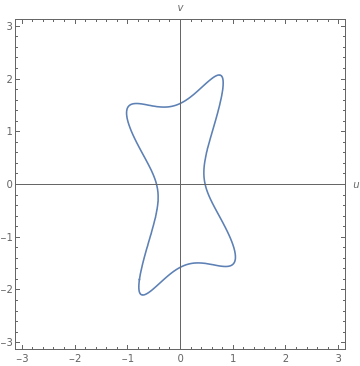
\includegraphics[width=4cm, height=4cm]{graphics/rational_1_oval.png}}\]
    \end{block}

\end{frame}

\section{Irrational Conic Bundles}

\subsection{Disconnected Real Loci}

\begin{frame}{Obstruction by Disconnected Real Loci}
\begin{itemize}
    \item Recall that if $\Ydd$ is $\Rbb$-rational, then $\Ydd(\Rbb)$ is \txtblue{connected} and non-empty.
    \item What if we take $\Ydd(\Rbb)$ to be \txtblue{disconnected}?
\end{itemize}
    The key insight is looking at $\pi_1(\Rbb): \Ydd(\Rbb) \to \Pbb^1_{[t_0 : t_1]}(\Rbb)$:
\begin{itemize}
    % \item \textbf{General Topological Fact: } It turns out that $\pi_1(\Rbb)$ is a continuous close map where every fiber is connected. This implies that
\end{itemize}
    \[\Ydd(\Rbb) \text{ is disconnected} \iff \pi_1(\Ydd(\Rbb)) \text{ is disconnected}\]
\end{frame}

\begin{frame}{Key Observation}
\begin{block}{Observation:}
    Take any point ${\color{red} [a: b]} \in \Pbb^1_{[t_0: t_1]}(\Rbb)$, then fiber of ${\color{red} [a: b]}$ is exactly the solutions satisfying:
   \[z^2 = Q_1(u, v, w){\color{red}(a)^2} + 2Q_2(u, v, w){\color{red}(ab)} + Q_3(u, v, w){\color{red}(b)^2}\]
   This equation has a solution if and only if the matrix
   \[M_{[a: b]} \coloneqq {\color{red}
\left[\begin{array}{@{}c|c@{}}
  \begin{matrix}
    M_1a^2 + 2M_2ab + M_3b^2
  \end{matrix}
  & 0 \\
\hline
  0 &
  \begin{matrix}
  -1
  \end{matrix}
\end{array}\right]
   }\] is \textbf{NOT} negative definite, where $M_1, M_2, M_3$ are the symmetric matrices associated to $Q_1, Q_2, Q_3$ respectively.
\end{block}
\end{frame}

\begin{frame}{Key Observation (Continued)}
    We will denote the signature of a real symmetric matrix $M$ as $(p, n)$, where $p$ is the number of positive eigenvalues and $n$ is the number of negative eigenvalues.

    \begin{block}{Lemma (Adapted from Degtjarev Et al., \cite{degtjarev_itenberg_kharlamov_2000})}
    Given the setup with $\Ydd$, let $M_{[t_0: t_1]}$ be the matrix defined the same as previously, then the signature of $M_{[t_0: t_1]}$ can only change by $\pm 1$ at real solutions of a degree $6$ polynomial\footnote{It is possible that one of the roots is the point at infinity, but we can without loss choose an appropriate basis to avoid this.}
    \[\Gamma(t) \coloneqq -det(M_1t^2 + 2M_2t + M_3)\]
    Notably, on each interval defined by real points of $\Gamma(t)$, the signature of $M_{[t_0: t_1]}$ stays the same.
    \end{block}
    %Appendix A4.2 of Real Enriques Surfaces by Alexander Degtyarev, Ilia Itenberg, Viatcheslav Kharlamov https://link.springer.com/book/10.1007/BFb0103960
\end{frame}

\begin{frame}{Disconnected Examples}
    Now, as long as we can find examples where at least two non-adjacent intervals with signature $(0, 4)$, this will produce a disconnected $\Ydd(\Rbb)$.
\begin{block}{Irrational Example with $\Delta(\Rbb)$ $3$ ovals}
Define $Q_1 \coloneqq  -u^2 - v^2 - w^2$, $Q_2 \coloneqq u^2 + 5v^2 + 9w^2$, and $Q_3 \coloneqq -24v^2 - 80w^2$. Then we have that
\[\Gamma(t) = t^6 - 30t^5 + 340t^4 - 1800t^3 + 4384t^2 - 3840t\] with $6$ real roots
\[t = 0, 2, 4, 6, 8, 10\]
\end{block}    
\end{frame}


\begin{frame}{Disconnected Examples}
\begin{block}{Example (Continued)}
    The signatures of $M_{[t_0: t_1]}$ follow the pattern:
    \[(0, 4), (1, 3), (0, 4), (1, 3), (0, 4), (1, 3)\]
    \[\frame{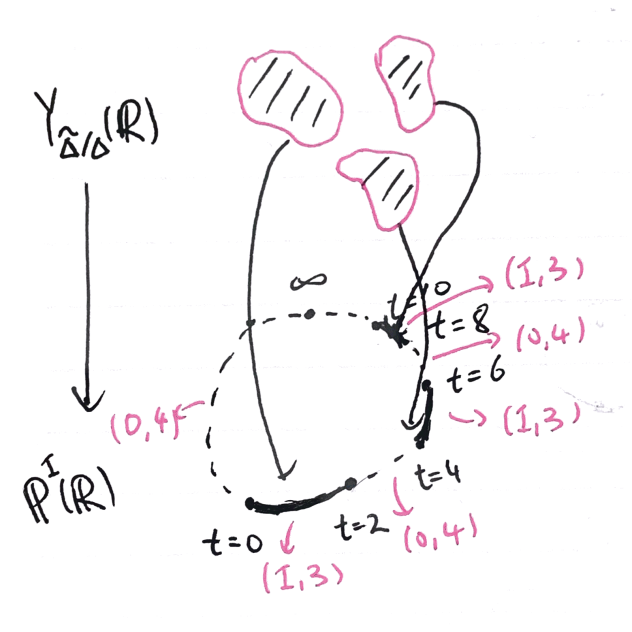
\includegraphics[width=5cm, height=5cm]{graphics/pi_1.png}}\]
\end{block}    
\end{frame}

% \begin{frame}{Disconnected Examples}
% \begin{block}{Example (Continued)}
%     This is the image of $\Ydd(\Rbb)$ under $\pi_2$:
%     \[\frame{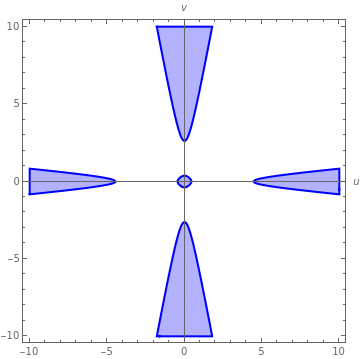
\includegraphics[width=5cm, height=5cm]{graphics/discon_3_oval.png}}\]
%     We see that it also has 3 connected components.
% \end{block}  
% \end{frame}

% \begin{frame}{The Explicit Construction}
%     The choice of $Q_1, Q_2, Q_3$ in the previous example may seem arbitrary, but you can ``reverse engineer" the appropriate $Q_1, Q_2, Q_3$ by considering
%     \[
% \begin{bmatrix}
% a_0 t^2 + b_0 t + c_0 & 0 & 0\\
% 0 & a_1 t^2 + b_1 t + c_1 & 0\\
% 0 & 0 & a_2 t^2 + b_2 t + c_2
% \end{bmatrix}
%     \]
%     \[= t^2(M_1) + t(2M_2) + M_3\]
%     and compare the coefficients.
% \end{frame}

\begin{frame}{Limitations of the Topological Obstruction}
    During the REU, we also showed that
    \begin{block}{Proposition:}
        If $\Ydd(\Rbb)$ is disconnected, then $\Delta(\Rbb)$ is either 2 non-nested ovals, 2 nested ovals, or 3 ovals. More precisely,
        \begin{itemize}
            \item $\Ydd(\Rbb)$ has at most $3$ connected components
            \item If $\Ydd(\Rbb)$ has $2$ connected components, then $\Delta(\Rbb)$ is either 2 non-nested ovals or 2 nested ovals
            \item If $\Ydd(\Rbb)$ has $3$ connected components, then $\Delta(\Rbb)$ is 3 ovals.
        \end{itemize}
    \end{block}
    Each case described above does occur.
\end{frame}

% \begin{frame}
% \begin{block}{Remark:}
%     % When $\Ydd(\Rbb)$ has $3$ connected components, the signatures of $\pi_1(\Rbb)$ has to be
%     % \[(0, 4), (1, 3), (0, 4), (1, 3), (0, 4), (1, 3)\]
%     When $\Ydd(\Rbb)$ has $2$ connected components, the signatures of $\Ydd(\Rbb)$ is one of
%     \begin{enumerate}
%         \item $(0, 4), (1, 3), (0, 4), (1, 3), (2, 2), (1, 3)$
%         \item $(0, 4), (1, 3), (0, 4), (1, 3)$
%     \end{enumerate}
% \vspace{\baselineskip}
%     If pattern $(1)$ occurs, then $\Delta(\Rbb)$ is 2 nested ovals.\\
% \vspace{\baselineskip}
% If pattern $(2)$ occurs, $\Delta(\Rbb)$ has always been $2$ non-nested ovals experimentally. \txtblue{It's unknown if the pattern $(2)$ implies that $\Delta(\Rbb)$ is $2$ non-nested ovals}.
% \end{block}
% \end{frame}

\subsection{Empty Real Loci}

\begin{frame}{The Case where $\Ydd(\Rbb) = \emptyset$}
\begin{itemize}
    \item Recall that if $\Ydd$ is $\Rbb$-rational, then $\Ydd(\Rbb)$ is connected and \txtblue{non-empty}.
    \item What if we take $\Ydd(\Rbb)$ to be \txtblue{empty} instead?
\end{itemize}

\begin{block}{Irrational Example where $\Delta(\Rbb) = \emptyset$}
    Define $Q_1 \coloneqq  -2u^2 - 3v^2 - 5w^2$, $Q_2 \coloneqq u^2 + 2v^2 + 3w^2$, and $Q_3 \coloneqq -2u^2 - 4v^2 - 2w^2$. Then one can verify that the associated $\Delta(\Rbb)$ and $\Ydd(\Rbb)$ are both empty, hence $\Ydd$ is irrational over $\Rbb$.
\end{block}
    This doesn't get us really far, as \txtblue{$\Ydd(\Rbb) = \emptyset$ implies that $\Delta(\Rbb) = \emptyset$}.
\end{frame}

\subsection{Irrational One Oval Example}

\begin{frame}{Irrational One Oval}

\begin{block}{Question:}
    What about the case for one oval?
\end{block}

S. Frei, L. Ji, S. Sankar, B. Viray, and I. Vogt showed that
\begin{block}{Irrational Example (Theorem 1.3(2), \cite{FJSVV})}
    Define $Q_1 \coloneqq  -u^2 - v^2 - 3w^2$, $Q_2 \coloneqq 3u^2 + 5v^2$, and $Q_3 \coloneqq -7u^2 - 23v^2 - 12w^2$, then $\Delta(\Rbb)$ is one oval, and the associated $\Ydd$ is irrational over any subfield of $\Rbb$.
\end{block}

% The main idea that this is irrational hinged on the fact that
% \begin{itemize}
%     \item $(Q_1 Q_3 - Q_2^2 < 0)_{\Rbb}$ is non-orientable
%     \item $\pi_1$ is not surjective on real points
% \end{itemize}

%The main idea behind showing this is irrational relied on what's known as an Intermediate Jacobian Torsor (IJT) obstruction.


    
\end{frame}

% \subsection{The Outlier}

% \begin{frame}{Four Ovals: The Outlier}
%     \begin{block}{Question:}
%         What about the case when $\Delta(\Rbb)$ is four ovals?
%     \end{block}
    
%     Based on ideas in collaboration previously with S. Frei,  S. Sankar,  B. Viray,  and I. Vogt, Lena Ji showed that
%     \begin{block}{Theorem:}
%         If $\Delta(\Rbb)$ is four ovals, then $\Ydd$ is $\Rbb$-rational.
%     \end{block}
% \end{frame}

\begin{frame}{Acknowledgements}
We would like to thank
\begin{itemize}
    \item Lena Ji for advising this project
    \item Sarah Frei, Soumya Sankar, Bianca Viray, and Isabel Vogt for helpful discussions and conversations 
    \item János Kollár for the question that motivated this project
    \item The University of Michigan Mathematics REU Program
    \item The National Science Foundation (Karen Smith’s NSF grant DMS-2101075) for funding this project
    \item My letter of recommendation writers Nicole Looper and Jungang Li
\end{itemize}

\end{frame}

\begin{frame}[allowframebreaks]
\frametitle{References}
% bibliography style is set to alpha here. you can experiment with other styles
\bibliographystyle{alpha}
% this line includes all references cited in the document. 
\bibliography{references.bib}
\end{frame}
\end{document}